\documentclass[11pt,a4paper]{article}
\usepackage[T1]{fontenc}
\usepackage[utf8]{inputenc}
\usepackage[margin=2.4cm]{geometry}
\usepackage{amsmath,amssymb,bm}
\usepackage{booktabs}
\usepackage{graphicx}
\usepackage{siunitx}
\sisetup{group-separator={\,},output-decimal-marker={,}}
\usepackage{tikz}
\usetikzlibrary{arrows.meta,calc,decorations.pathreplacing,patterns,positioning}
\usepackage{listings}
\usepackage{xcolor}
\usepackage[colorlinks=true,linkcolor=blue!45!black,citecolor=blue!45!black]{hyperref}


\renewcommand{\figurename}{Figura}
\renewcommand{\tablename}{Tabela}
\renewcommand{\contentsname}{Sumário}
\renewcommand{\refname}{Referências}

\newcommand{\bxt}{b_{\mathrm{xt}}}
\newcommand{\bat}{b_{\mathrm{at}}}
\newcommand{\thi}{\theta_{\mathrm{inc}}}
\newcommand{\rhor}{\rho_{r}}
\newcommand{\uhat}{\hat{\bm{u}}}

\lstset{
  basicstyle=\ttfamily\small, keywordstyle=\color{blue!55!black},
  commentstyle=\color{green!35!black}\itshape, stringstyle=\color{orange!70!black},
  numbers=left, numberstyle=\tiny\color{gray}, frame=single, framerule=0.3pt,
  rulecolor=\color{gray!50}, breaklines=true, showstringspaces=false,
  language=Python, xleftmargin=1.6em, framexleftmargin=1.6em
}

\title{\bfseries Co-registro em range entre canais\\[2mm]
\large O termo que falta na reconstrução multicanal em azimute}
\author{Notas técnicas --- projeto SATA2D}
\date{Setembro de 2026}

\begin{document}
\maketitle

\begin{abstract}
\noindent
A reconstrução multicanal em azimute do \texttt{sata2d} corrige a \emph{fase}
de cada canal receptor através dos coeficientes $C_0$, $C_1$, $C_2$, e o SATA
remove o resíduo topográfico $\delta C_0$. Nenhum desses termos toca a
\emph{posição} do envelope comprimido em range. Um receptor deslocado de
$\bxt$ na direção cross-track enxerga o alvo num slant range mais curto, e
essa diferença --- \SI{38.5}{m}, ou \num{1.47} células de range, no preset
padrão --- permanece não corrigida. Somar canais com envelopes desalinhados
custa correlação, e isso trava a reconstrução em \SI{96}{\percent} do pico
monostático independentemente de quão perfeito seja o modelo de fase. Este
documento deduz o termo, quantifica sua magnitude, mostra por que ele é
insensível à topografia (ao contrário da fase) e apresenta a implementação
via teorema do deslocamento.
\end{abstract}

\tableofcontents
\bigskip\hrule

% ==========================================================================
\section{O problema, em uma medida}
% ==========================================================================

O ponto de partida é um experimento numérico. Constrói-se um filtro de
reconstrução \emph{oráculo}: em vez de assumir a terra plana na altura $h_0$,
ele recebe a altura verdadeira do alvo, de modo que $C_0$, $C_1$ e $C_2$
ficam todos exatos. É o limite superior de qualquer melhoria possível no
modelo de fase.

\begin{table}[h]
\centering
\begin{tabular}{lrrr}
\toprule
caso & pico & \% do monostático & erro/sinal in-band \\
\midrule
referência monostática & \num{1.314e4} & \SI{100.0}{\percent} & --- \\
sem SATA               & \num{1.052e3} & \SI{8.0}{\percent}   & \SI{+1.18}{dB} \\
SATA (só $C_0$)        & \num{1.254e4} & \SI{95.4}{\percent}  & \SI{-6.39}{dB} \\
\textbf{oráculo (altura verdadeira)} & \num{1.263e4} & \textbf{\SI{96.1}{\percent}} & \textbf{\SI{-6.27}{dB}} \\
\bottomrule
\end{tabular}
\caption{Fase perfeita não resolve. O oráculo ganha \num{0.7} ponto
percentual sobre o SATA com $C_0$ apenas, e \emph{nada} em erro/sinal.}
\end{table}

\noindent
A conclusão é forte: os \SI{4}{\percent} que faltam \textbf{não são um
problema de fase}. Este documento mostra que são um problema de
\emph{atraso}.

% ==========================================================================
\section{Geometria e notação}
% ==========================================================================

Trabalhamos em coordenadas SAR: $x$ ao longo da trajetória (azimute), $y$
cross-track horizontal, $z$ altura. Para um sistema de um transmissor e
$N_{rx}$ receptores:
\begin{align}
\bm{p}_{tx}(t) &= (v t,\; 0,\; H) \\
\bm{p}_{rx,i}(t) &= (v t + b_{\mathrm{at},i},\; b_{\mathrm{xt},i},\; H) \\
\bm{p} &= (x_0,\; y_0,\; h) \qquad \text{(alvo)}
\end{align}

O caminho de ida e volta do canal $i$ e o seu \emph{meio-caminho} --- que é a
grandeza que a compressão em range posiciona no eixo de atraso --- valem
\begin{equation}
r_{bs,i}(t) = \|\bm{p}_{tx}(t)-\bm{p}\| + \|\bm{p}_{rx,i}(t)-\bm{p}\|,
\qquad
R_i(t) = \tfrac{1}{2}\, r_{bs,i}(t).
\label{eq:Ri}
\end{equation}
A referência monostática é $R_{mono}(t) = \|\bm{p}_{tx}(t)-\bm{p}\|$.

No instante de centro de feixe $t_{bc}$ (aproximação máxima, em broadside
$v t_{bc} = x_0$) define-se
\begin{equation}
r = \|\bm{p}_{tx}(t_{bc})-\bm{p}\| = \sqrt{y_0^2 + (H-h)^2},
\qquad
\sin\thi = \frac{y_0}{r},
\qquad
\cos\thi = \frac{H-h}{r},
\end{equation}
e o versor de linha de visada plataforma$\to$alvo é
\begin{equation}
\uhat = \frac{\bm{p}-\bm{p}_{tx}(t_{bc})}{r} = \bigl(0,\; \sin\thi,\; -\cos\thi\bigr).
\label{eq:uhat}
\end{equation}

\begin{figure}[h]
\centering
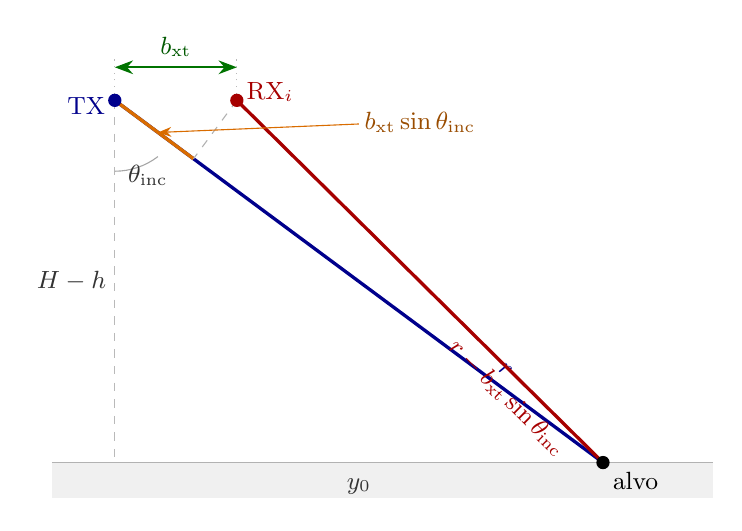
\begin{tikzpicture}[scale=1.0,>=Stealth]
  \def\H{4.6}      \def\Y{6.2}
  \coordinate (T)  at (0,\H);
  \coordinate (R)  at (1.55,\H);
  \coordinate (P)  at (\Y,0);
  \coordinate (N)  at (0,0);
  % ground
  \fill[gray!12] (-0.8,-0.45) rectangle (\Y+1.4,0);
  \draw[gray!60] (-0.8,0) -- (\Y+1.4,0);
  % nadir
  \draw[gray!55,dashed] (T) -- (N);
  % rays
  \draw[very thick,blue!55!black] (T) -- (P) node[pos=0.78,above,sloped,font=\small]{$r$};
  \draw[very thick,red!65!black]  (R) -- (P) node[pos=0.78,below,sloped,font=\small]{$r-\bxt\sin\thi$};
  % angle
  \draw[gray!70] ($(T)!0.9cm!(N)$) arc (-90:-52.5:0.9cm);
  \node[font=\small,gray!40!black] at (0.42,\H-0.95) {$\thi$};
  % baseline
  \draw[<->,thick,green!45!black] (T) ++(0,0.42) -- ++(1.55,0)
      node[midway,above,font=\small,green!35!black]{$\bxt$};
  \draw[gray!55,dotted] (T) -- ++(0,0.55);
  \draw[gray!55,dotted] (R) -- ++(0,0.55);
  % projection of bxt on the LOS
  \coordinate (Q) at ($(T)!(R)!(P)$);
  \draw[very thick,orange!85!black] (T) -- (Q);
  \draw[gray!60,dashed] (R) -- (Q);
  \draw[orange!85!black,->,thin] (3.1,\H-0.30) -- ($(T)!0.55!(Q)$);
  \node[orange!60!black,font=\small,anchor=west] at (3.05,\H-0.28) {$\bxt\sin\thi$};
  % markers
  \fill[blue!55!black] (T) circle (2.4pt) node[left,font=\small,yshift=-2pt]{TX};
  \fill[red!65!black]  (R) circle (2.4pt) node[right,font=\small,yshift=3pt]{RX$_i$};
  \fill[black] (P) circle (2.4pt) node[below right,font=\small]{alvo};
  \node[font=\small,gray!40!black] at (-0.55,\H/2) {$H-h$};
  \node[font=\small,gray!40!black] at (\Y/2,-0.3) {$y_0$};
\end{tikzpicture}
\caption{Geometria cross-track no centro de feixe. O deslocamento $\bxt$ do
receptor projeta-se na linha de visada como $\bxt\sin\thi$: a perna de
recepção encurta exatamente disso. Como o meio-caminho é a média das duas
pernas e só uma delas se move, o envelope desloca-se de $\bxt\sin\thi/2$.}
\label{fig:geom}
\end{figure}

% ==========================================================================
\section{Dedução do termo}
% ==========================================================================

\subsection{Perturbação de primeira ordem}

Escreva $\bm{p}_{tx}(t_{bc}) - \bm{p} = -r\,\uhat$ e seja
$\bm{b} = (\bat,\, \bxt,\, 0)$ o deslocamento do receptor. Então
\begin{equation}
\|\bm{p}_{rx}-\bm{p}\| = \bigl\| -r\uhat + \bm{b} \bigr\|
= r\sqrt{1 - \frac{2\,\bm{b}\cdot\uhat}{r} + \frac{\|\bm{b}\|^2}{r^2}}.
\end{equation}
Expandindo a raiz para $\|\bm{b}\| \ll r$,
\begin{equation}
\boxed{\;\|\bm{p}_{rx}-\bm{p}\| \;=\; r \;-\; \underbrace{\bm{b}\cdot\uhat}_{\text{1\textsuperscript{a} ordem}}
\;+\; \underbrace{\frac{\|\bm{b}\|^2 - (\bm{b}\cdot\uhat)^2}{2r}}_{\text{2\textsuperscript{a} ordem}}
\;+\; \mathcal{O}\!\left(\frac{b^3}{r^2}\right).}
\label{eq:expansao}
\end{equation}

\subsection{Por que a baseline along-track não aparece}

Este é o passo que faz o termo ser tão simples. Substituindo
\eqref{eq:uhat}:
\begin{equation}
\bm{b}\cdot\uhat
= \underbrace{\bat \cdot 0}_{=\,0} + \bxt\sin\thi + 0\cdot(-\cos\thi)
= \bxt \sin\thi .
\label{eq:proj}
\end{equation}
A componente $x$ de $\uhat$ é \emph{exatamente zero} no centro de feixe ---
essa é a definição de aproximação máxima, a linha de visada é perpendicular
à trajetória. Portanto $\bat$ não contribui em primeira ordem para o
deslocamento em range. O que $\bat$ faz é deslocar o \emph{instante} de
centro de feixe,
\begin{equation}
\Delta t_i = \frac{b_{\mathrm{at},i}}{2v},
\end{equation}
que é o offset temporal DPCA --- já contabilizado pela reconstrução através
do coeficiente $Dt$. São dois efeitos ortogonais: $\bat$ mexe em azimute,
$\bxt$ mexe em range.

\subsection{O resultado}

De \eqref{eq:Ri}, \eqref{eq:expansao} e \eqref{eq:proj}, o deslocamento do
meio-caminho do canal $i$ em relação à referência monostática é
\begin{equation}
\boxed{\;
\Delta R_i(r) \;=\; R_i - R_{mono}
\;=\; -\,\frac{b_{\mathrm{xt},i}\,\sin\thi(r)}{2}
\;+\; \frac{b_{\mathrm{at},i}^2 + b_{\mathrm{xt},i}^2\cos^2\thi}{4\,r}
\;+\;\cdots
\;}
\label{eq:dR}
\end{equation}
com
\begin{equation}
\sin\thi(r) = \frac{\sqrt{r^2 - (H-h)^2}}{r}.
\end{equation}
O fator $1/2$ vem de \eqref{eq:Ri}: apenas uma das duas pernas do caminho
bistático se move.

\subsection{Verificação numérica}

A Tabela~\ref{tab:verif} compara \eqref{eq:dR} truncada em primeira ordem
contra o cálculo exato de \eqref{eq:Ri} sobre as trajetórias reais do preset
padrão ($\lambda=\SI{0.25}{m}$, $H=\SI{720}{km}$, $r_0=\SI{766.206}{km}$,
$\thi=\SI{20}{\degree}$, $N_{rx}=4$, $\bat=[0,100,200,300]\,$m,
$\bxt=[-225,-75,75,225]\,$m, $\rhor = \SI{26.11}{m}$).

\begin{table}[h]
\centering
\begin{tabular}{crrrrr}
\toprule
ch & $\bxt$ [m] & $\Delta R$ exato [m] & 1\textsuperscript{a} ordem [m] & erro [cm] & erro [bins] \\
\midrule
0 & $-225$ & \num{0.000}   & \num{0.000}   & ---  & --- \\
1 & $-75$  & $-\num{25.727}$ & $-\num{25.715}$ & \num{1.1} & \num{0.0004} \\
2 & $+75$  & $-\num{51.437}$ & $-\num{51.431}$ & \num{0.6} & \num{0.0002} \\
3 & $+225$ & $-\num{77.132}$ & $-\num{77.146}$ & \num{1.5} & \num{0.0006} \\
\bottomrule
\end{tabular}
\caption{A fórmula fechada reproduz a geometria bistática exata com erro
$\le\SI{1.5}{cm}$, consistente com o termo de segunda ordem de
\eqref{eq:dR} (poucos cm para estas baselines). Excursão total
ch0$\to$ch3: \SI{77.1}{m} $=$ \num{2.95} bins, ou $\pm\num{1.47}$ em torno
do centro.}
\label{tab:verif}
\end{table}

% ==========================================================================
\section{Fase \emph{versus} envelope: a separação de escalas}
% ==========================================================================

Este é o ponto conceitual do documento. O sinal comprimido em range do canal
$i$ tem a forma
\begin{equation}
s_i(\tau) \;=\;
\underbrace{\exp\!\left(-j\,\frac{4\pi R_i}{\lambda}\right)}_{\text{portadora}}
\;\cdot\;
\underbrace{w\!\left(\tau - \frac{2R_i}{c}\right)}_{\text{envelope}} .
\label{eq:sinal}
\end{equation}
O \emph{mesmo} $R_i$ aparece nos dois fatores, mas com escalas de
sensibilidade radicalmente diferentes: a portadora responde na escala de
$\lambda = \SI{0.25}{m}$, o envelope na escala de $\rhor = \SI{26.11}{m}$.
A razão é
\begin{equation}
\frac{\rhor}{\lambda} \;\approx\; 100 .
\end{equation}

É útil separar $\Delta R_i$ em duas parcelas:
\begin{equation}
\Delta R_i \;=\;
\underbrace{\Delta R_i^{\mathrm{geom}}}_{\text{baseline, terra plana}}
\;+\;
\underbrace{\delta R_i^{\mathrm{topo}}}_{\text{correção de altura}},
\end{equation}
e ver o que cada uma faz em cada fator.

\subsection{A parcela geométrica}

$\Delta R^{\mathrm{geom}} = -\bxt\sin\thi/2 = \SI{38.5}{m}$ para o canal
extremo. Na \textbf{fase} isso vale
$4\pi\cdot\num{38.5}/\num{0.25} = \num{1935}$~rad --- enorme, mas
perfeitamente \emph{conhecido} e já aplicado pelo filtro via $C_0$. No
\textbf{envelope} vale \num{1.47} bins --- e não é corrigido por ninguém.
\textbf{É este o termo que falta.}

\subsection{A parcela topográfica}

Derivando $\sin\thi = y/r$ com $y = \sqrt{r^2-(H-h)^2}$ a $r$ fixo,
\begin{equation}
\frac{\partial \sin\thi}{\partial h}
= \frac{1}{r}\frac{\partial y}{\partial h}
= \frac{1}{r}\cdot\frac{H-h}{y}
= \frac{\cos\thi}{r\sin\thi},
\end{equation}
logo
\begin{equation}
\delta R^{\mathrm{topo}}
= -\frac{\bxt}{2}\cdot\frac{\cos\thi}{r\sin\thi}\,\delta h .
\label{eq:topo}
\end{equation}
Para $\delta h = \SI{240}{m}$ e $\bxt = \SI{225}{m}$ isso dá
$\SI{9.7}{cm}$. Na \textbf{fase} são \SI{278}{\degree} de \emph{erro} (o
filtro assumiu terra plana) --- é exatamente o que o SATA remove. No
\textbf{envelope} são \num{0.0037} bins --- irrelevante.

\begin{table}[h]
\centering
\begin{tabular}{lrrl}
\toprule
parcela & fase & envelope & quem corrige \\
\midrule
$\Delta R^{\mathrm{geom}} = \SI{38.5}{m}$ & \num{1935} rad (conhecida) & \textbf{\num{1.47} bins} & $C_0$ / \textbf{ninguém} \\
$\delta R^{\mathrm{topo}} = \SI{9.7}{cm}$ & \textbf{\SI{278}{\degree} de erro} & \num{0.0037} bins & \textbf{SATA} / --- \\
2\textsuperscript{a} ordem $\approx \SI{4.4}{cm}$ & \SI{126}{\degree} & \num{0.0017} bins & $C_0$ numérico / --- \\
\bottomrule
\end{tabular}
\caption{A mesma geometria, quatro efeitos. Em negrito, o que precisa de
correção. Note que o co-registro é o único item cuja fase já está resolvida
e cujo envelope não está.}
\label{tab:matriz}
\end{table}


\begin{figure}[h]
\centering
\includegraphics[width=\textwidth]{envelopes.pdf}
\caption{Os quatro envelopes comprimidos em range de um mesmo alvo, no
preset padrão. À esquerda como chegam à reconstrução: deslocados de
$\delta_i = \Delta R_i/\rhor = \pm\num{1.47}$ e $\pm\num{0.49}$ amostras em
relação à grade monostática. À direita depois da rampa
\eqref{eq:rampa}. A fase de portadora é idêntica nos dois painéis --- é o
envelope, e só ele, que se move.}
\label{fig:env}
\end{figure}

\subsection{Duas consequências práticas}

\begin{enumerate}
\item \textbf{O co-registro não precisa de DEM.} Por \eqref{eq:topo}, a
sensibilidade do envelope à topografia é \num{0.0037} bins para
$\SI{240}{m}$ de altura. Basta a geometria de terra plana e a baseline. Isso
o torna muito mais barato que o SATA, que precisa de um modelo de terreno
justamente porque atua na escala de $\lambda$.

\item \textbf{Corrigir a fase não move o envelope.} É por isso que o oráculo
da Seção~1 empacou nos mesmos \SI{96.1}{\percent}: ele conserta o primeiro
fator de \eqref{eq:sinal} e deixa o segundo intocado. Somar $N_{rx}$
envelopes deslocados é perda de correlação, e nenhum modelo de fase desfaz
isso.
\end{enumerate}

% ==========================================================================
\section{A correção: teorema do deslocamento}
% ==========================================================================

\subsection{Derivação}

Queremos mover o envelope do canal $i$ de $\tau_i = 2R_i/c$ para
$\tau_0 = 2R_{mono}/c$, ou seja, construir
\begin{equation}
g_i(\tau) \;=\; s_i\!\left(\tau + \frac{2\Delta R_i}{c}\right).
\end{equation}
Verificação: $g_i$ tem seu pico onde $\tau + 2\Delta R_i/c = \tau_i$, isto é
em $\tau = \tau_i - 2\Delta R_i/c = \tau_0$. Correto.

Pelo par de Fourier $s(\tau - a) \leftrightarrow S(f)\,e^{-j2\pi f a}$, com
$a = -2\Delta R_i/c$:
\begin{equation}
\boxed{\;
S_i^{\mathrm{coreg}}(f_r) \;=\; S_i(f_r)\cdot
\exp\!\left(+\,j\,\frac{4\pi f_r\, \Delta R_i}{c}\right)
\;}
\label{eq:rampa}
\end{equation}

\subsection{A armadilha: $f_r$ tem que ser banda-base}

Em \eqref{eq:rampa}, $f_r$ é a frequência de range \textbf{relativa à
portadora} $f_0$, não absoluta. A razão está em \eqref{eq:sinal}: o
deslocamento que queremos é do envelope apenas. Se usarmos $f_0 + f_r$, o
fator extra é
\begin{equation}
\exp\!\left(j\,\frac{4\pi f_0 \Delta R_i}{c}\right)
= \exp\!\left(j\,\frac{4\pi \Delta R_i}{\lambda}\right),
\end{equation}
que é \emph{exatamente} a fase de portadora que $C_0$ já aplicou. Para o
canal 3 isso vale $-\num{55411}\si{\degree}$ de contagem dupla --- a
reconstrução seria destruída. A rampa banda-base move o envelope e deixa a
portadora intacta: é precisamente a divisão de trabalho desejada.

\subsection{Forma discreta}

Em bins de FFT, com $N$ amostras de range e passo
$\rhor = c/(2 f_s)$, o deslocamento em amostras é
\begin{equation}
\delta_i \;=\; \frac{2\Delta R_i}{c}\,f_s \;=\; \frac{\Delta R_i}{\rhor}
\;=\; -\,\frac{b_{\mathrm{xt},i}\sin\thi}{2\,\rhor},
\end{equation}
e a rampa fica
\begin{equation}
\mathrm{ramp}[k] \;=\; \exp\!\left(j\,2\pi\,\frac{k - N/2}{N}\,\delta_i\right),
\qquad k = 0,\dots,N-1
\end{equation}
(com o \texttt{fftshift} adequado à ordenação da FFT). Para o canal 3:
$\delta_3 = -\num{38.48}/\num{26.11} = -\num{1.474}$ amostras.

Esta é literalmente a mesma construção do passo \texttt{residual BC shifts}
do SATA2D em IDL --- lá com \texttt{ramp = 2*!pi*j*(findgen(Nzp\_rg) -
Nzp\_rg/2)/Nzp\_rg}. A diferença é só de onde vem $\delta$.

\subsection{Parte inteira e parte fracionária}

Para $|\delta_i| \lesssim 2$ amostras, como aqui, a rampa sozinha basta e o
efeito de \emph{wraparound} da convolução circular fica confinado às bordas
do swath. Para deslocamentos maiores convém separar
\begin{equation}
\delta_i = \underbrace{\lfloor \delta_i \rceil}_{\text{\texttt{roll} inteiro}}
\;+\; \underbrace{\bigl(\delta_i - \lfloor \delta_i \rceil\bigr)}_{\text{rampa}},
\end{equation}
que é o que o SATA2D faz com o MoCo de centro de feixe.

% ==========================================================================
\section{Dependência em range e em azimute}
% ==========================================================================

\subsection{Em range: quase constante}

$\thi$ varia ao longo do swath, logo $\Delta R_i$ também. No preset padrão:

\begin{table}[h]
\centering
\begin{tabular}{lrrr}
\toprule
& $r$ [km] & $\thi$ [\si{\degree}] & $\Delta R$ para $\bxt=\SI{225}{m}$ [m] \\
\midrule
near  & \num{765.538} & \num{19.862} & $-\num{38.22}$ \\
mid   & \num{766.206} & \num{20.000} & $-\num{38.48}$ \\
far   & \num{768.851} & \num{20.534} & $-\num{39.46}$ \\
\bottomrule
\end{tabular}
\caption{Variação total de \SI{1.24}{m} $=$ \num{0.0475} bins ao longo do
swath.}
\end{table}

\noindent
Menos de \num{0.05} bin: \textbf{um escalar por canal, avaliado em
$r_{ref}$, é suficiente}. O critério geral é
\begin{equation}
\frac{\bxt}{2\rhor}\bigl[\sin\thi(r_{far}) - \sin\thi(r_{near})\bigr]
\;\lesssim\; 0.1 \ \text{bin}.
\end{equation}
Quando isso falhar (swath largo, $\bxt$ grande), a solução é a mesma do
SATA2D: blocos curtos em range, FFT curta por bloco, rampa com
$\thi(r_n)$, overlap-add. O código já existe.

\subsection{Em azimute: constante --- e isso está medido}

O deslocamento acima foi derivado no centro de feixe. Ao longo da abertura,
a diferença de histórias de range entre canais poderia variar --- é o termo
diferencial de RCM. Sua assinatura é exatamente o coeficiente $C_2$, e a
medida é:

\begin{table}[h]
\centering
\begin{tabular}{crrrrrr}
\toprule
ch & $\delta C_0$ [mm] & $\delta C_1$ [mm/s] & $\delta C_2$ [mm/s\textsuperscript{2}]
   & $\varphi_0$ & $\varphi_1$ (pp) & $\varphi_2$ (borda) \\
\midrule
0 & \num{193.344} & $-\num{0.0000}$ & $-\num{0.0000}$ & \SI{278.4}{\degree} & \SI{0.000}{\degree} & \SI{0.000}{\degree} \\
1 & \num{64.452}  & \num{0.0000}    & $-\num{0.0000}$ & \SI{92.8}{\degree}  & \SI{0.000}{\degree} & \SI{0.000}{\degree} \\
2 & $-\num{64.457}$ & $-\num{0.0000}$ & \num{0.0000}  & \SI{-92.8}{\degree} & \SI{0.000}{\degree} & \SI{0.000}{\degree} \\
3 & $-\num{193.383}$ & $-\num{0.0000}$ & \num{0.0000} & \SI{-278.5}{\degree} & \SI{0.000}{\degree} & \SI{0.000}{\degree} \\
\bottomrule
\end{tabular}
\caption{Resíduos dos coeficientes,
$\delta C_k = C_k(\text{alvo real}) - C_k(\text{ponto flat no mesmo range})$,
convertidos em fase sobre $T_{int}=\SI{2.155}{s}$. As razões são
$|\varphi_1|/|\varphi_0| = \num{2.7e-8}$ e
$|\varphi_2|/|\varphi_0| = \num{2.4e-9}$: ruído numérico do \texttt{polyfit}.}
\label{tab:coef}
\end{table}

\noindent
$\delta C_2 = 0$ significa que as curvaturas de RCM dos canais são idênticas
--- portanto \textbf{um escalar por canal, constante em azimute, basta}.

A razão de $C_1 \equiv 0$ é geométrica: em broadside com trajetórias retas e
paralelas, tanto $r_{ms}(t)$ quanto $r_{bs}(t)$ são funções \emph{pares} em
torno dos seus respectivos pontos de aproximação máxima. Após o alinhamento
em $t_{bc}$, a diferença $r_{bs}-r_{ms}$ não tem termo ímpar. Elevar o alvo
preserva a simetria, então o resíduo também é nulo. \emph{Isto deixa de valer
sob squint} --- ali $C_1$ e $C_2$ voltam a ter conteúdo, e a rampa passa a
precisar de dependência em azimute.

% ==========================================================================
\section{Implementação}
% ==========================================================================

\subsection{Onde entra}

Logo após a compressão em range dos dados de canal e \textbf{antes} de
\texttt{reconstruct\_subband\_2d}: a inversão multicanal pressupõe que todos
os canais amostram o mesmo alvo na mesma célula de range. É independente do
SATA (um atua em fase, o outro em atraso) e os dois comutam em primeira
ordem.

\begin{center}
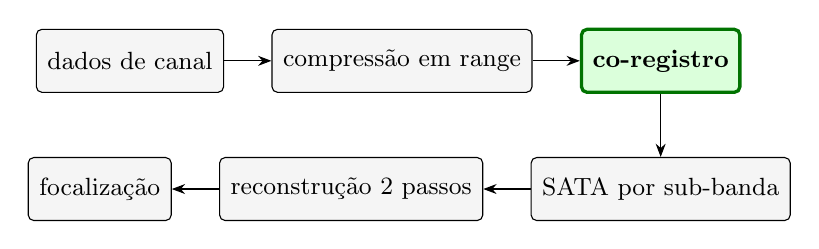
\begin{tikzpicture}[node distance=6mm,>=Stealth,every node/.style={font=\small}]
  \tikzset{blk/.style={draw,rounded corners=2pt,inner sep=4pt,minimum height=8mm,fill=gray!8},
           new/.style={draw,rounded corners=2pt,inner sep=4pt,minimum height=8mm,
                       fill=green!14,draw=green!45!black,very thick}}
  \node[blk] (a) {dados de canal};
  \node[blk,right=of a] (b) {compressão em range};
  \node[new,right=of b] (c) {\textbf{co-registro}};
  \node[blk,below=8mm of c] (d) {SATA por sub-banda};
  \node[blk,left=of d] (e) {reconstrução 2 passos};
  \node[blk,left=of e] (f) {focalização};
  \draw[->] (a)--(b); \draw[->] (b)--(c);
  \draw[->] (c.south)--(d.north);
  \draw[->] (d)--(e); \draw[->] (e)--(f);
\end{tikzpicture}
\end{center}

\subsection{Esboço}

\begin{lstlisting}
def coregister_range(s_ch, p, tracks, r_ref=None):
    """s_ch: [Nrx, Na_ch, Nr] range-compressed channel data.

    Desloca o envelope de cada canal para a grade monostatica.
    Nao toca na fase de portadora -- a rampa e' banda-base.
    """
    Nr = s_ch.shape[-1]
    rho_r = C_LIGHT / (2.0 * p.rsf)
    r_ref = p.r0 if r_ref is None else r_ref
    sin_th = np.sqrt(max(r_ref**2 - (p.H - p.h0)**2, 0.0)) / r_ref

    # frequencia de range BANDA-BASE, na ordenacao da FFT
    k = np.fft.fftfreq(Nr) * Nr            # -Nr/2 .. Nr/2-1, unshifted

    out = np.empty_like(s_ch)
    for i in range(p.Nrx):
        dR = -p.bxt[i] * sin_th / 2.0      # [m]  Eq. (13)
        delta = dR / rho_r                 # [amostras]
        ramp = np.exp(2j * np.pi * k * delta / Nr)
        out[i] = np.fft.ifft(np.fft.fft(s_ch[i], axis=-1) * ramp, axis=-1)
    return out
\end{lstlisting}

\noindent
Notas:
\begin{itemize}
\item \texttt{np.fft.fftfreq(Nr)*Nr} devolve o índice de frequência já na
ordenação não-deslocada da FFT, o que evita um par de \texttt{fftshift}.
\item O sinal de \texttt{delta} segue \eqref{eq:rampa}; se o pico andar para
o lado errado, é o sinal desta linha (e vale conferir com um alvo pontual
sintético antes de rodar a cena toda).
\item Para swath largo, trocar o escalar \texttt{sin\_th} por
$\sin\thi(r_n)$ dentro de um laço de blocos de range.
\end{itemize}

% ==========================================================================
\section{Validação esperada}
% ==========================================================================

A evidência de que este é o termo dominante vem de uma varredura em $\bxt$
com o filtro oráculo --- fase exata, de modo que o único resíduo é o
desalinhamento:

\begin{table}[h]
\centering
\begin{tabular}{rrrrr}
\toprule
dxt [m] & $\bxt^{\max}$ [m] & desalinhamento [bins] & pico oráculo & erro/sinal \\
\midrule
\num{150} & \num{225} & \num{1.47} & \SI{96.1}{\percent} & \SI{-6.27}{dB} \\
\num{30}  & \num{45}  & \num{0.29} & \SI{99.4}{\percent} & \SI{-9.17}{dB} \\
\num{5}   & \num{8}   & \num{0.05} & \SI{99.8}{\percent} & \SI{-19.50}{dB} \\
\bottomrule
\end{tabular}
\caption{Monotônico no desalinhamento. A última linha é o piso imposto por
todos os outros efeitos juntos.}
\label{tab:sweep}
\end{table}

\noindent
Com o co-registro implementado a $\bxt = \SI{225}{m}$, a expectativa é
aproximar-se da última linha: \textbf{$\sim\SI{99}{\percent}$ de pico e
erro/sinal na casa dos $\SI{-15}{dB}$ a $\SI{-20}{dB}$}. Isso ainda precisa
ser medido --- a tabela acima isola o efeito, mas não é prova de que a
correção o remove por completo.

\subsection{O que não é corrigido}

\begin{itemize}
\item \textbf{Desalinhamento residual dependente de azimute} sob squint,
quando $\delta C_1, \delta C_2 \neq 0$.
\item \textbf{Migração de célula de range} dentro da abertura: o co-registro
alinha os canais entre si no centro de feixe; a RCM comum a todos continua
sendo tarefa do RCMC.
\item \textbf{Decorrelação volumétrica} para $\bxt$ muito grande --- um
limite físico, não algorítmico.
\end{itemize}

% ==========================================================================
\section{Resumo}
% ==========================================================================

\begin{enumerate}
\item Um receptor deslocado de $\bxt$ vê o alvo a
$\Delta R = -\bxt\sin\thi/2$ de distância. No preset: \SI{38.5}{m}, ou
\num{1.47} células de range.
\item A baseline along-track $\bat$ não contribui em primeira ordem, porque
$\uhat$ é perpendicular à trajetória no centro de feixe. Ela produz o offset
temporal $\bat/2v$, que já é tratado.
\item Esse deslocamento aparece na fase (via $C_0$, já corrigido) \emph{e}
no envelope (não corrigido). A separação de escalas $\rhor/\lambda \approx
100$ é o que torna os dois problemas independentes.
\item A correção é uma rampa linear na frequência de range \textbf{banda-base}
--- e usar frequência absoluta duplicaria $C_0$.
\item No preset, um escalar por canal basta: a variação ao longo do swath é
\num{0.05} bin e a sensibilidade à topografia é \num{0.004} bin.
\item Isso é ortogonal a $C_1$/$C_2$, que são identicamente nulos em
broadside e portanto não têm nada a oferecer.
\end{enumerate}

\end{document}
